\chapter{Descripción del Modelo} \label{chap:modelo}
% CAP 2 descripción del modelo. qué se resuelve, método numérico. Explicación de FEM
% podría ir teoría de gradientes conjugados, etc

% section con explicación de todo el trabajo (solo teoría, nada de imple). debería ir con las fórmulas y todo. podría ir dibujito de célula con ángulo \theta
%\subsection{Potencial eléctrico}

% El chapter anterior debería tener una explicación a grandes rasgos de que es lo que se hace en el trabajo

%Primero tiene que ir una introducción a grandes rasgos de lo que se hace (revisar chapter intro)

En este capítulo se explica en detalle el modelo matemático estudiado y los métodos numéricos utilizados para resolverlo.

\section{Modelo Matemático}

Se estudia una única célula idealizada de forma esférica y compuesta por dos materiales: el líquido intracelular (citoplasma) y una fina membrana celular. La célula se encuentra sumergida en un líquido conductor extracelular, y se aplican pulsos eléctricos por medio de dos electrodos equidistantes a ella, con una diferencia de potencial constante. Los electrodos se encuentran en los bordes superior e inferior del dominio. A lo largo del trabajo se utiliza la letra $E$ para representar el campo eléctrico, $\alpha$ para el radio de la célula y $\theta$ para el ángulo polar.

%\begin{figure}[h]
%	\centering
%	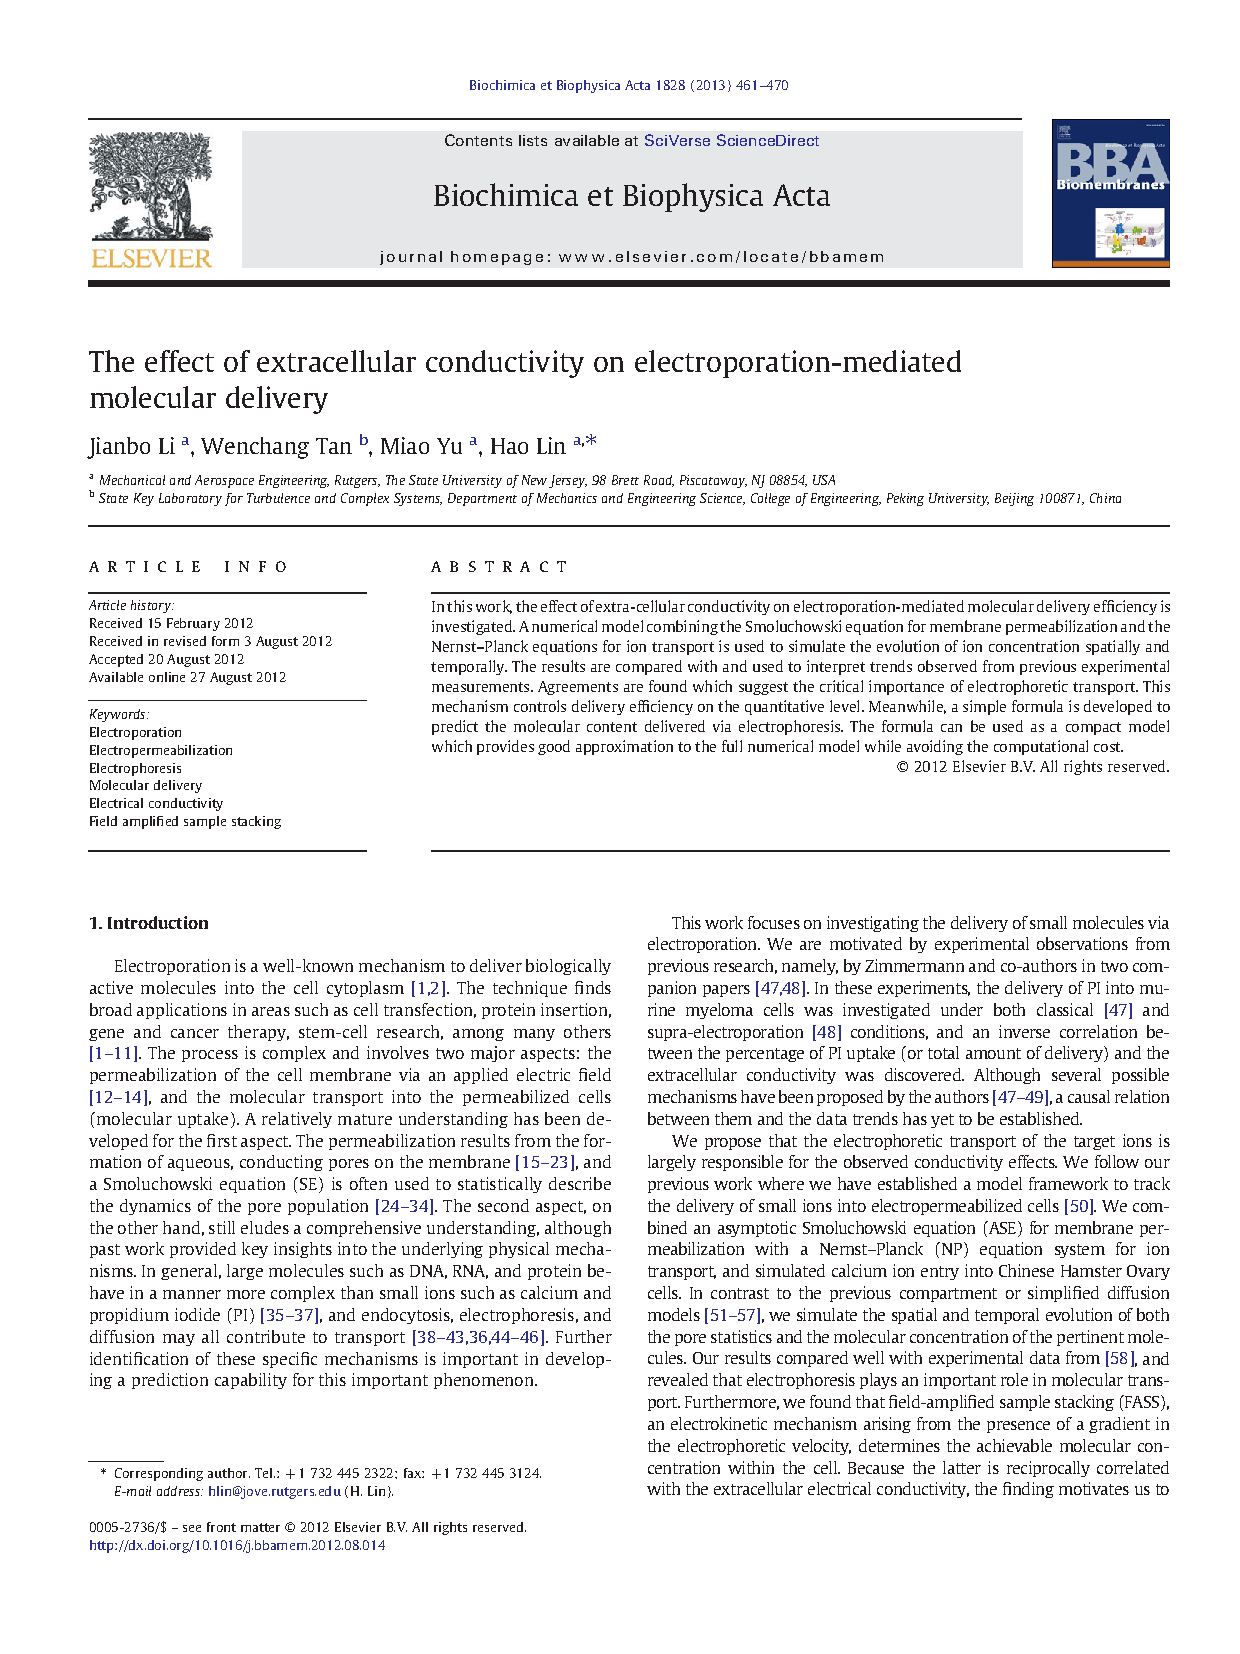
\includegraphics[width=0.40\linewidth]{celula}
%	\caption{PTM en función del tiempo en distintos ángulos polares para dos potenciales aplicados diferentes}
%	\label{fig:itv-time}
%\end{figure}

%\begin{figure}[h]
%\floatbox[{\capbeside\thisfloatsetup{capbesideposition={right,top},capbesidewidth=4cm}}]{figure}[\FBwidth]
%{\caption{A test figure with its caption side by side}\label{fig:test}}
%{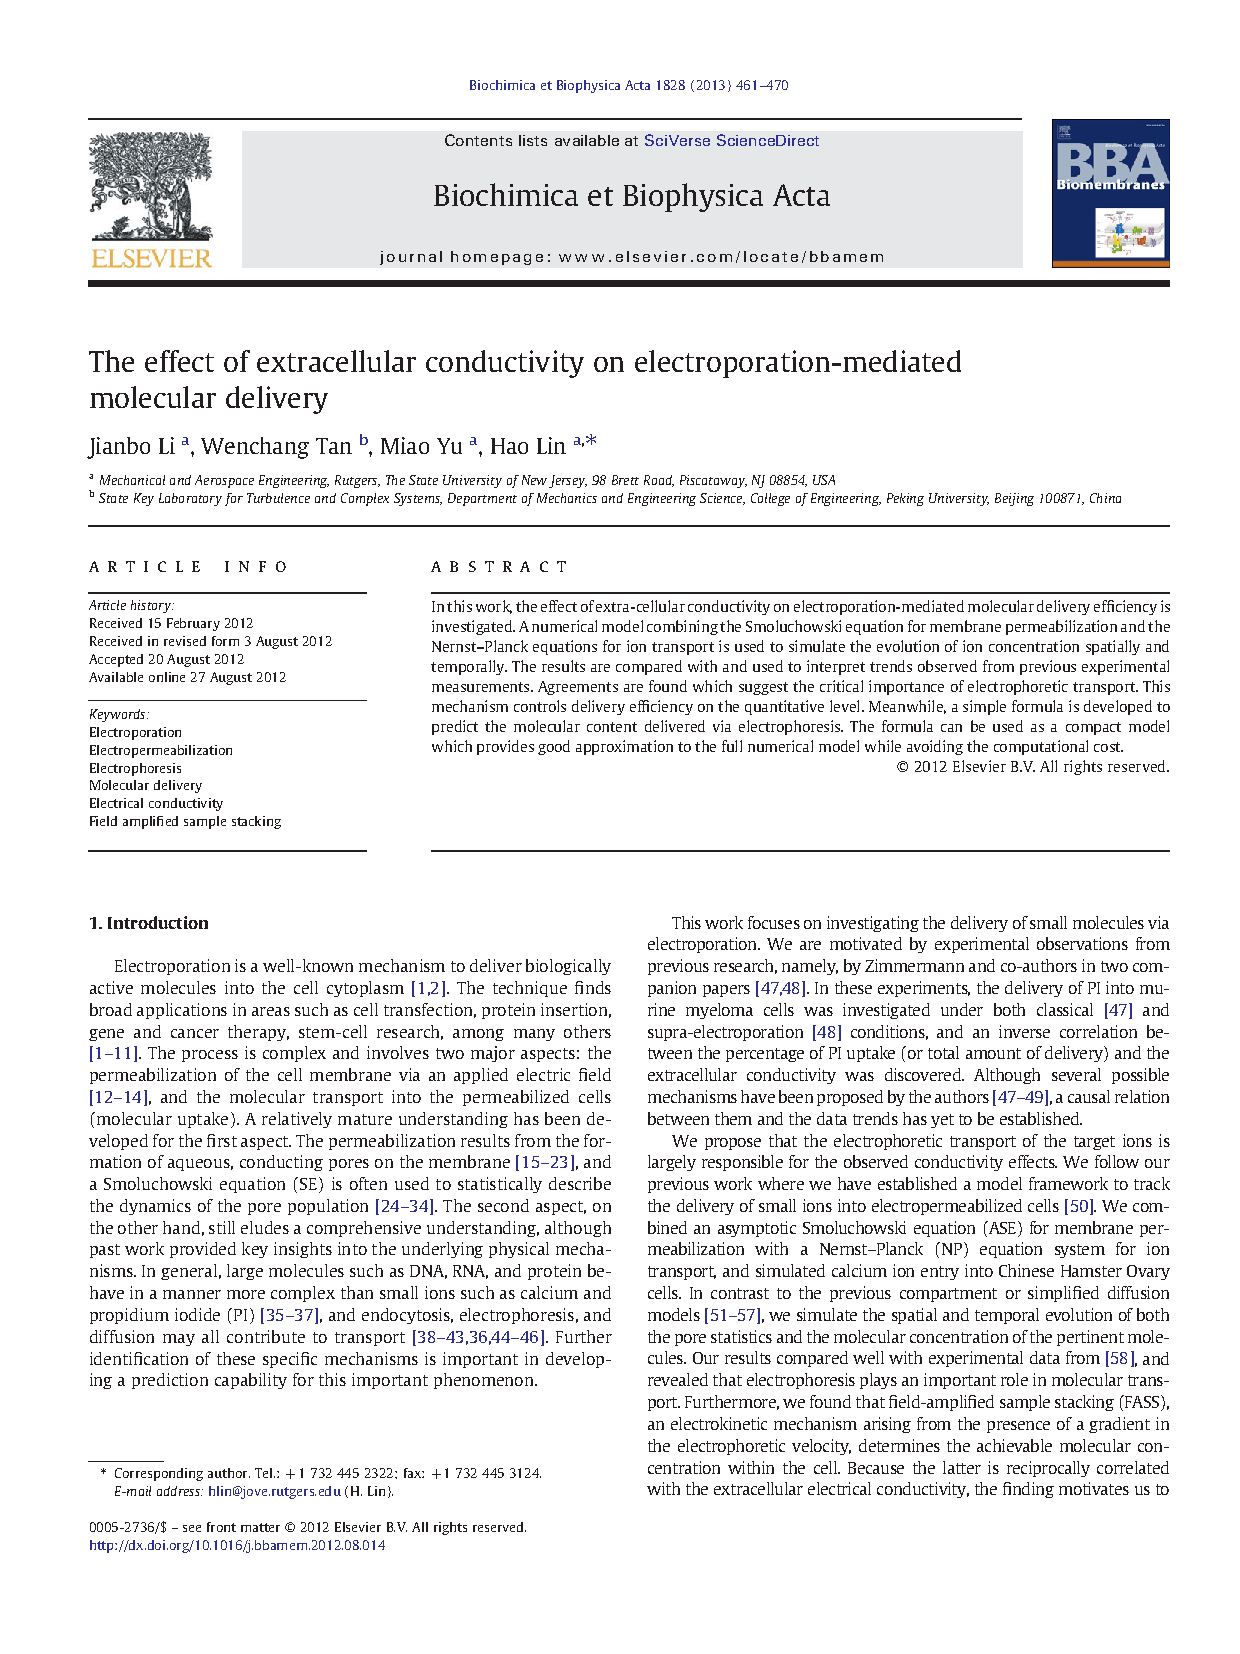
\includegraphics[width=5cm]{celula}}
%\end{figure}

%\begin{figure}[h]
%  \begin{minipage}[r]{0.50\textwidth}
%    \includegraphics[width=\textwidth]{dominio2}
%  \end{minipage}\hfill
%  \begin{minipage}[l]{0.5\textwidth}
%    \caption{
%       Modelo de la célula de radio $r$.\\ $\theta$ representa el ángulo polar\\ y $E$ el campo eléctrico.
%    } \label{fig:03-03}
%  \end{minipage}
%\end{figure}

\begin{figure}[hb]
	\centering
	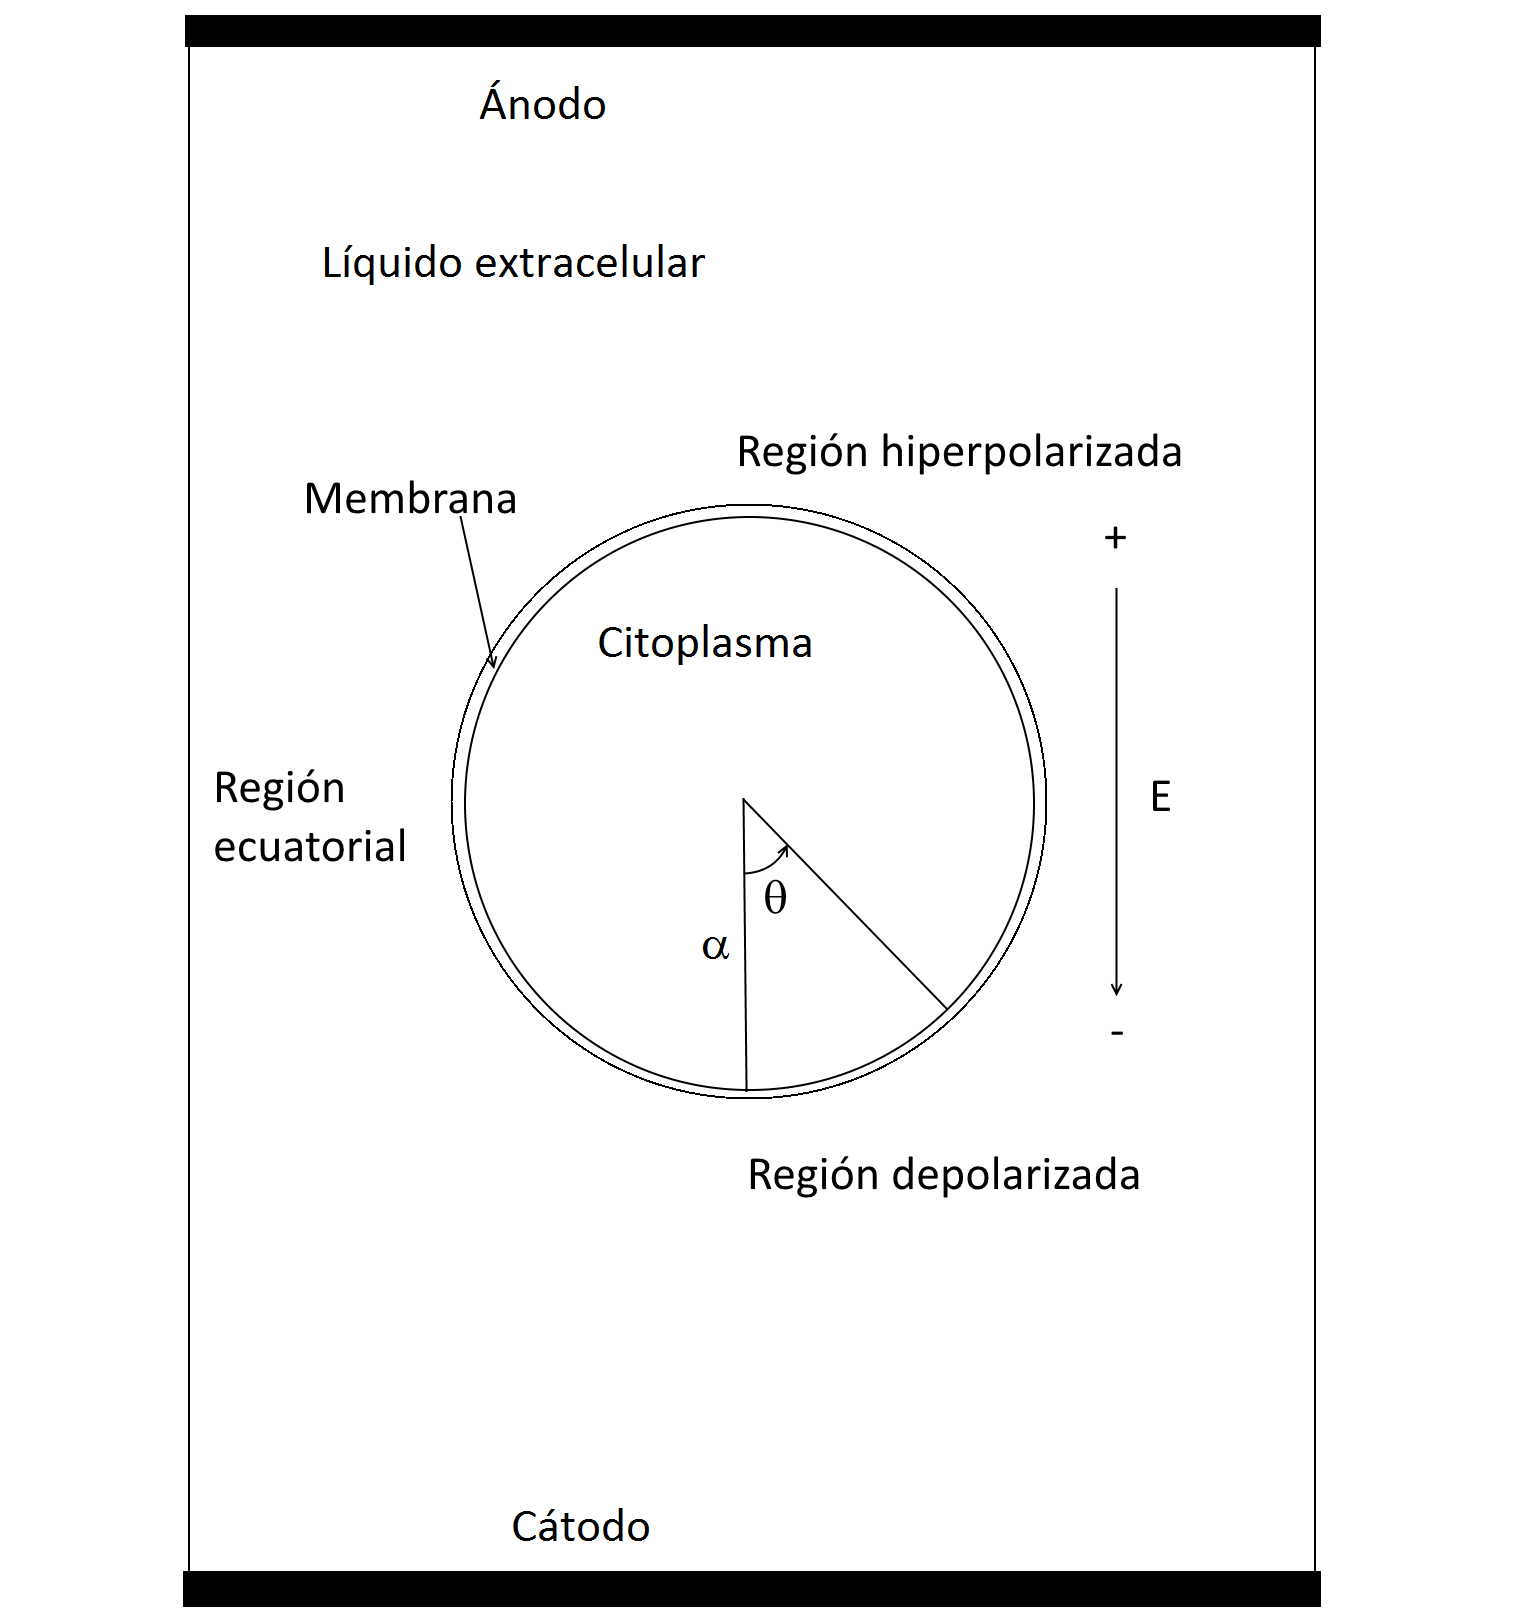
\includegraphics[scale=0.30]{dominio}
	\label{fig:dominio}
	\caption{Dominio del problema}
\end{figure}

\clearpage

Los pulsos se dividen en dos partes con un tiempo de encendido (\ontime) en el que la diferencia de potencial es constante y un tiempo de apagado (\offtime) sin diferencia de potencial entre los electrodos.

\begin{figure}[h]
	\centering
	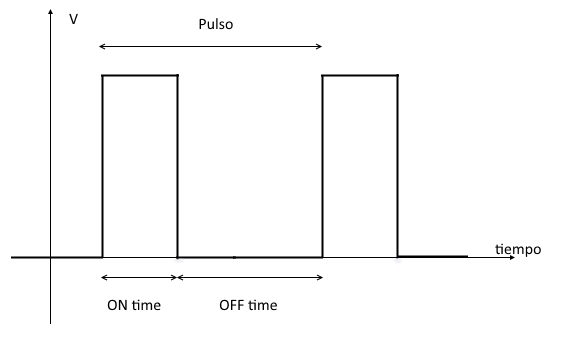
\includegraphics[scale=0.75]{pulso}
\end{figure}


\subsection*{Potencial Eléctrico}
El potencial eléctrico generado por los electrodos se calcula en todo el dominio según la ecuación de Laplace \cite{c9-fem-electro}

\begin{equation} \label{eq:poisson}
	\nabla \sigma_{elem} \cdot (\nabla \phi) = 0 
\end{equation}

donde $\phi$ representa el potencial eléctrico y $\sigma_{elem}$ la conductividad del material, para $elem = o, i$ o $m$ para el líquido extracelular, el citoplasma o la membrana celular respectivamente. Los valores de las conductividades son muy diferentes para los tres tipos de material, siendo en particular la conductividad de la membrana celular mucho menor que la del resto del dominio.

La diferencia de potencial entre el interior y el exterior de la célula en un punto de su superficie se conoce como potencial transmembrana (PTM). Si la célula es esférica este potencial se puede aproximar con la fórmula cerrada \cite{tsong}

\begin{equation} \label{eq:cos}
	 V^{\theta} = f_s\, E\, \alpha\, \cos (\theta) 
\end{equation}

con

\begin{equation} \label{eq:lambda}
    f_s = \frac{3\sigma_o \left( 3 d \alpha^2 \sigma_i + \left( 3 d^2 \alpha - d^3 \right) \left(\sigma_m - \sigma_i \right) \right)}{2 \alpha^3 \left( \sigma_m + 2 \sigma_o \right) \left(\sigma_m + \frac{1}{2} \sigma_i \right) - 2 \left(\alpha - d \right)^3 \left(\sigma_o - \sigma_m \right) \left( \sigma_i - \sigma_m \right)}
\end{equation}

donde $E$ es el campo eléctrico, $\theta$ el ángulo polar respecto del campo eléctrico, $\alpha$ el radio de la célula y $\sigma_o$, $\sigma_i$ y $\sigma_m$ las conductividades del líquido extracelular, intracelular y de la membrana respectivamente. Cuando el valor de $\sigma_m$ es al menos cinco órdenes de magnitud menor que $\sigma_o$ y $\sigma_i$, el valor de $f_s$ se puede aproximar como $3/2$\cite{c5-puchiar}. La fórmula \ref{eq:cos} no tiene en cuenta que el PTM puede variar en el tiempo por la creación de poros, por eso en este trabajo no se la usa directamente, si no que usa la ecuación \ref{eq:poisson}.

\subsection*{Generación y evolución de poros}
El PTM genera en la membrana celular la aparición de poros hidrofílicos, cuya variación de la densidad de poros en el tiempo se puede describir según la ecuación diferencial ordinaria \cite{krass-viejo}

\begin{equation} \label{eq:poros-crea}
	\frac{\partial N}{\partial t} = \alpha_c e^{(V_m/V_{ep})^2} \left( 1 - \frac{N}{N_0 e^{q \left(V_m/V_{ep} \right) ^2}} \right)
\end{equation}

%poner cita \cite{krass}
donde $N$ es la densidad de poros en un determinado tiempo y posición de la membrana celular, $\alpha_c$ es el coeficiente de creación de poros, $V_m$ es el potencial transmembrana, $V_{ep}$ es el voltaje característico de electroporación, $N_0$ es la densidad de poros en equilibrio (cuando $V_m = 0$) y $q$ es una constante igual a $(r_m / r*)^2$, donde $r_m$ es el radio de mínima energía para $V_m = 0$ y $r*$ es el radio mínimo de los poros. Esta ecuación se usa para cada región de la membrana por separado, ya que depende del PTM, que no es constante en la superficie. 

Los poros se crean con un radio inicial $r*$ y su radio varía en el tiempo según el potencial transmembrana de acuerdo a la ecuación diferencial ordinaria \cite{krass07}

\begin{equation} \label{eq:poros-radio}
	\frac{\partial r}{\partial t} = \frac{D}{kT} \left( \frac{V_m^2 F_{max}}{1+r_h / (r+r_a)} + \frac{4 \beta}{r} \left(\frac{r_*}{r}\right)^4 - 2 \pi \gamma + 2 \pi \sigma_{\textrm{\tiny eff}} r\right)
\end{equation}

donde $r$ es el radio de un poro, $D$ es el coeficiente de difusión para los poros, $k$ es la constante de Boltzmann, $T$ la temperatura absoluta, $V_m$ el potencial transmembrana, $F_{max}$ la máxima fuerza eléctrica para $V_m$ de 1V, $r_h$ y $r_a$ son constantes usadas para la velocidad de advección, $\beta$ es la energía de repulsión estérica, $\gamma$ es la energía del perímetro de los poros, y $\sigma_{\textrm{\tiny eff}}$ es la tensión efectiva de la membrana, calculada como

\begin{equation}
	\sigma_{\textrm{\tiny eff}} = 2 \sigma^\prime - \frac{2 \sigma^\prime - \sigma_0}{(1 - A_p / A)^2}
\end{equation}

% puede ir \cite{krass}
donde $\sigma^\prime$ es la tensión de la interfase hidrocarburo-agua, $\sigma_0$ es la tensión de la bicapa sin poros, $A_p$ es la suma de las áreas de todos los poros en la célula, y $A$ es el área de la célula. En la ecuación \ref{eq:poros-radio}, el primer término corresponde a la fuerza eléctrica inducida por el potencial transmembrana, el segundo a la repulsión estérica, el tercero a la tensión de línea que actúa en el perímetro del poro y el cuarto a la tensión superficial de la célula. Se debe analizar el radio de cada poro individualmente y no en conjunto.\\

Por otra parte se asume que la membrana celular se carga como un capacitor y una resistencia en paralelo. De esta manera el potencial transmembrana no aumenta bruscamente al iniciarse el pulso eléctrico, si no que crece de manera paulatina según la ecuación \cite{hibino}

\begin{equation} \label{eq:capacit} \begin{split}
	V_m = V_p\, (1 - e^{-t/\tau}) , \\ \textrm{con } \tau = \alpha\, C_m \left( \frac{1}{\sigma_i} + \frac{1}{2 \sigma_o} \right)
\end{split} \end{equation}

donde $V_m$ es el potencial transmembrana en un punto de la superficie de la célula, $V_p$ es el potencial obtenido por las ecuaciones de potencial eléctrico en ése mismo punto, $t$ es el tiempo transcurrido desde el comienzo del pulso eléctrico, $\alpha$ es el radio de la célula, $C_m$ es la capacitancia superficial de la célula y $\sigma_i$ y $\sigma_o$ las conductancias intra y extracelulares respectivamente.

\subsection*{Transporte de especies}
Se estudia el transporte de cuatro especies iónicas: \h, \oh, \na y \cl{} en el dominio. Para conocer las concentraciones en las diferentes regiones e instantes de tiempo se utiliza la ecuación de conservación de masa de Nernst-Planck \cite{c6-fodava}

%Para conocer la concentración de las especies iónicas se usa la ecuación de conservación de masa de Nernst-Planck \cite{c6-fodava}

\begin{equation} \label{eq:trans}
	\frac{\partial C_i}{\partial t} = \nabla \cdot \left( D_i \nabla C_i + D_i z_i \frac{F}{R T} C_i \nabla \phi \right)
\end{equation}

%\cite{fodava} abajo
donde $C_i$, $D_i$ y $z_i$ representan la concentración, el coeficiente de difusión y la valencia respectivamente de la especie $i$, para $i = $ \h, \oh, \na ó \cl.
$F$ es la constante de Faraday, $R$ la constante de los gases y $T$ la temperatura. 
Esta ecuación tiene en cuenta la difusión de las partículas (con el término $D_i \nabla C_i$) pero también el efecto de migración producto del campo eléctrico (con el término $D_i z_i \frac{F}{R T} C_i \nabla \phi$). 

\subsection*{Condiciones de borde}
Para la ecuación \ref{eq:poisson} se usan condiciones de borde de Dirichlet con potenciales fijos en los electrodos:

\begin{equation}
	\phi_a \; \textrm{para el ánodo y } \phi_c = 0 \; \textrm{para el cátodo}
\end{equation}


mientras que para el borde no ocupado por electrodos se usan condiciones de borde de Neumann:

\begin{equation}
	\frac{\partial \phi}{\partial \mathbf{n}} = 0
\end{equation}

donde $\mathbf{n}$ representa la normal al borde.\\

Para la ecuación de generación de poros \ref{eq:poros-crea} se usa como condición inicial que la membrana no contiene poros, mientras que para la ecuación \ref{eq:poros-radio} se asume que los poros se crean con un radio inicial $r^*$.

Para la ecuación de transporte de especies \ref{eq:trans} se usan como condiciones iniciales las concentraciones descritas en la tabla \ref{table:tablita}: $C_{e, i}^0$ siendo $e =$ $i$ ó $o$ si se refiere a los nodos del interior o del exterior de la célula respectivamente e $i =$ \h, \oh, \na ó \cl{} para la concentración de cada especie. %y $C_{e,i}$ con $e =$ $a$ ó $c$ si es para el ánodo o el cátodo respectivamente.

Como condición de borde en el borde no ocupado por los electrodos se usa

\begin{equation}
	\frac{\partial C_i}{\partial \mathbf{n}} = 0
\end{equation}

%Para los bordes ocupados por los electrodos se usan los valores fijos $C_{e,i}$ descritos anteriormente.

\clearpage
\subsection*{Constantes}
A continuación se presenta la definición y valores de las constantes usadas.

\newcommand{\lineaTabla}[3]{ ${#1}$ & {#3} & {#2} \\ }

\newcommand{\anodo}[3] {
	\lineaTabla{C_{a,{#1}}}{\num{#2} \si{#3}}{Concentración de #1 en el ánodo}
}

\newcommand{\catodo}[3] {
	\lineaTabla{C_{c,{#1}}}{\num{#2} \si{#3}}{Concentración de #1 en el cátodo}
}

\begin{table}[h!]
    \centering
	\begin{tabular}{|l l l|} 
		\hline Símbolo & Definición & Valor \\
		\hline
		\lineaTabla{\sigma_{o}}{0.20 \si{\siemens\per\metre}}{Conductividad de la zona extracelular}
		\lineaTabla{\sigma_{i}}{0.15 \si{\siemens\per\metre}}{Conductividad de la zona intracelular}
		\lineaTabla{\sigma_{m}}{\num{5e-6} \si{\siemens\per\metre}}{Conductividad de la membrana celular}
		\lineaTabla{\sigma_{p}}{2 \si{\siemens\per\metre}}{Conductividad del líquido que llena el poro}
		\lineaTabla{E}{1000\vcm - 2000\vcm}{Campo eléctrico aplicado}
		\lineaTabla{\alpha}{10 \si{\micro\metre} - 50 \si{\micro\metre}}{Radio de la célula}
		\lineaTabla{d}{5 \si{\nano\metre}}{Ancho de la membrana}
		
		\lineaTabla{D_{\h}}{\num{12500} \si{\micro\metre\per\metre^{2}}}{Coeficiente de difusión para \h}
		\lineaTabla{D_{\oh}}{\num{7050} \si{\micro\metre\per\metre^{2}}}{Coeficiente de difusión para \oh}
		\lineaTabla{D_{\na}}{\num{1780} \si{\micro\metre\per\metre^{2}}}{Coeficiente de difusión para \na}
		\lineaTabla{D_{\cl}}{\num{3830} \si{\micro\metre\per\metre^{2}}}{Coeficiente de difusión para \cl}	
		\lineaTabla{C_{i,\h}^0}{\num{.3978e-7} \si{\textsc{m}}}{Concentración inicial de \h{} en citoplasma}
		\lineaTabla{C_{i,\oh}^0}{\num{.3978e-7} \si{\textsc{m}}}{Concentración inicial de \oh{} en citoplasma}
		\lineaTabla{C_{i,\na}^0}{\num{142} \si{\milli\textsc{m}}}{Concentración inicial de \na{} en citoplasma}
		\lineaTabla{C_{i,\cl}^0}{\num{108} \si{\milli\textsc{m}}}{Concentración inicial de \cl{} en citoplasma}

		\lineaTabla{C_{o,\h}^0}{\num{1e-7} \si{\textsc{m}}}{Concentración inicial externa de \h}
		\lineaTabla{C_{o,\oh}^0}{\num{1e-7} \si{\textsc{m}}}{Concentración inicial externa de \oh}
		\lineaTabla{C_{o,\na}^0}{\num{14e-7} \si{\milli\textsc{m}}}{Concentración inicial externa de \na}
		\lineaTabla{C_{o,\cl}^0}{\num{4e-7} \si{\milli\textsc{m}}}{Concentración inicial externa de \cl}
	
	\begin{comment}
		\anodo{\h}{1.5e7}{at.\micro\metre^{-3}} 
		\anodo{\oh}{0}{}
		\anodo{\na}{1e12}{at.\micro\metre^{-3}}
		\anodo{\cl}{0}{}

		\catodo{\h}{0}{}
		\catodo{\oh}{1.806e7}{at.\micro\metre^{-3}}
		\catodo{\na}{0}{}
		\catodo{\cl}{0}{}
	\end{comment}
		
		\lineaTabla{r*}{0.51 \si{\nano\metre}}{Radio mínimo de los poros}
		\lineaTabla{r_m}{0.80 \si{\nano\metre}}{Radio del poro de mínima energía}
		\lineaTabla{\alpha_c}{\num{1e9} \si{\metre^{-2}\siemens^{-1}}}{Coeficiente de creación de poros}
		\lineaTabla{V_{ep}}{0.258 \si{\volt}}{Voltaje característico}
		\lineaTabla{N_0}{\num{1.5e9} \si{\metre^{-2}}}{Densidad de poros en equilibrio}
		\lineaTabla{D}{\num{5e-14} \si{\metre^{-2}\siemens^{-1}}}{Coeficiente de difusión para poros}
		\lineaTabla{F_{max}}{\num{0.7e-3} \si{\newton\volt^{-2}}}{Máxima fuerza eléctrica}
		\lineaTabla{r_h}{\num{0.97e-9} \si{\metre}}{Constante usada para la velocidad de advección}
		\lineaTabla{r_a}{\num{0.31e-9} \si{\metre}}{Constante usada para la velocidad de advección}
		\lineaTabla{\beta}{\num{1.4e19} \si{\joule}}{Repulsión estérica}
		\lineaTabla{\gamma}{\num{1.8e11} \si{\joule\per\metre}}{Energía del perímetro de los poros}
		\lineaTabla{\sigma^\prime}{\num{2e-2} \si{\joule\metre^{-2}}}{Tensión de la interfase hidrocarburo-agua}
		\lineaTabla{\sigma_0}{\num{1e-6} \si{\joule\metre^{-2}}}{Tensión de la bicapa sin poros}
		\lineaTabla{C_m}{\num{1e-14} \si{\farad\metre^{-2}}}{Capacitancia superficial de la célula}

		\lineaTabla{F}{\num{9.648534} \si{\coulomb\per\mole}}{Constante de Faraday}
		\lineaTabla{R}{\num{8.3144621} \si{\joule\per\coulomb\per\mole}}{Constante de los gases}
		\lineaTabla{T}{310 \si{\kelvin}}{Temperatura}
		\lineaTabla{k}{\num{1.3806488e-23} \si{\joule\per\kelvin}}{Constante de Boltzmann}
		
		\hline
	\end{tabular} 
	\caption{Valores constantes usados.Valores obtenidos de  \cite{c4-marino}, \cite{c5-puchiar} y \cite{krass07}}
	\label{table:tablita}
\end{table}

\newpage

\section{Métodos Computacionales}

%Las ecuaciones descritas en la sección anterior fueron resueltas utilizando los métodos numéricos de elementos finitos y diferencias finitas. 

La complejidad de las ecuaciones descritas en la sección anterior obliga a resolverlas con métodos numéricos. Se eligieron los métodos de elementos finitos y diferencias finitas, que fueron totalmente desarrollados en este trabajo. El método de elementos finitos requiere además resolver sistemas de ecuaciones lineales, los cuales se resolvieron utilizando la librería Eigen \cite{eigen}.

\subsection*{Método de Elementos Finitos}

El método de elementos finitos (FEM, \textit{Finite Element Method}) es una herramienta computacional que se utiliza para resolver ecuaciones diferenciales discretizando el dominio en zonas pequeñas llamadas elementos y resolviendo un sistema de ecuaciones lineales con el que se obtiene la solución de las ecuaciones diferenciales en un conjunto de puntos del dominio. Una ventaja del método es que permite modelar con facilidad dominios con formas complejas, y que permite enfocar la atención en zonas del dominio que sean de particular interés, o que contengan cambios bruscos en la solución del problema, modelando sin problemas con elementos de tamaño variable. La aplicación del método de elementos finitos consiste en \cite{zien, gouri}:

\begin{itemize}
	\item Discretizar el dominio continuo en una malla formada por elementos unidos por nodos. Cada uno de estos elementos debe ser pequeño y tener una forma simple (por ejemplo triángulos o cuadriláteros si el dominio es bidimensional). El conjunto de elementos debe ser disjunto y ocupar todo el dominio; es decir, cada punto del dominio debe estar ocupado por uno y sólo un elemento. Los vértices de los elementos se llaman nodos, y suelen ser un punto en común entre dos o más elementos. Cuántos más pequeños sean los elementos, mayor será la precisión de la solución al aplicar el método, pero se necesitarán más elementos para cubrir el dominio, y por lo tanto un mayor poder de cómputo. 

	\item Definir funciones de forma. Una función de forma  de un nodo de un elemento es una función tal que vale 1 cuando se evalúa en el nodo que la define, 0 cuando se evalúa en los demás nodos del elemento, y tiene valores intermedios para los demás puntos del interior. 

	\item Plantear la ecuación $R(e) = \int_{v} N \cdot (L(u) + f_v)\, dv$  para cada elemento, donde la ecuación diferencial a resolver tiene la forma $L(u) + f_v = 0$, $N$ es un vector con las funciones de forma definidas anteriormente, y $R(e)$ es el residuo del elemento, que se intentará minimizar. Luego igualar el residuo a 0 y obtener un sistema de ecuaciones lineales de la forma $K u = f$ donde $K$ es una matriz de $n_e \times n_e$, con $n_e$ la cantidad de nodos por elemento, $u$ es el vector con los valores nodales de la ecuación a resolver y $f$ es un vector de longitud $n_e$. La matriz $K$ del sistema generado se denomina matriz de rigidez, y el vector $f$ vector de fuerza. Para llegar al sistema de ecuaciones lineales suele ser necesario usar integración por partes para reducir el orden de las ecuaciones diferenciales y puede ser necesario resolver integrales con métodos aproximados de integración numérica. La manera de llegar al sistema de ecuaciones lineales depende de la ecuación diferencial a resolver, del tipo de los elementos usados y de las funciones de forma elegidas. 
	
	\item Ensamblar todos los sistemas de ecuaciones elementales en un sistema grande, con tantas ecuaciones e incógnitas como nodos en la malla. El valor en cada nodo debe ser igual para los diferentes elementos a los que pertenece. El proceso de ensamblaje se realiza reescribiendo cada sistema elemental obtenido en el punto anterior por un sistema global, de $n \times n$, donde cada elemento de la matriz de rigidez $K$ se coloca en la posición correspondiente al nodo que representa según la numeración global de los nodos en todo el dominio, y el resto de los elementos se dejan en 0. Luego se suman todas las matrices globales de cada elemento para obtener una única matriz global de rigidez del sistema. Lo mismo se debe realizar con el vector de fuerza $f$. La cantidad de elementos distintos de cero en cada fila $i$ de la matriz de rigidez depende de la cantidad de elementos a los que pertenece el nodo $i$ en la malla que representa el dominio y de la cantidad de nodos por elemento.
	
	\item Agregar las condiciones de borde al sistema global. En algunos casos es posible realizar este paso al generar las ecuaciones elementales, es decir antes de ensamblar el sistema. Diferentes condiciones de borde se agregan de diferentes maneras. Por ejemplo la condición de borde de Dirichlet en un nodo $i$ se puede agregar al sistema reemplazando la fila $i$ de la matriz de rigidez por una fila con 1 en la posición $i$ y ceros en las demás posiciones, y reemplazando el valor en la posición $i$ del vector de fuerza por el valor indicado por la condición de borde. 
	
	\item Resolver el sistema ensamblado con algún método de resolución de ecuaciones lineales. El vector $u$ global obtenido contiene las soluciones en los nodos de la ecuación diferencial. Dado que la matriz ensamblada es muy poco densa (muy pocos elementos distintos de cero), se suele representar con estructuras especiales para matrices dispersas. Si la matriz de rigidez global $K$ es simétrica definida positiva\footnote{$K$ es simétrica definida positiva si $K = K^\intercal$ y $x^\intercal K x > 0$ para todo vector $x \neq 0$} se pueden utilizar métodos especiales como descomposición de Cholesky, LDL o gradientes conjugados, que pueden reducir sustancialmente los tiempos de cómputo. También se pueden reducir los tiempos de resolución si se tiene una matriz banda\footnote{$K$ es una matriz con banda $p$ si $K_{ij} = 0 \; \forall j < i-p$ ó $j > i+p$, es decir todos los valores distintos de cero están dentro de una banda diagonal con un ancho conocido} de rigidez. Para lograr esto último es necesario haber asignado números a los nodos de la malla de manera tal que se minimice la máxima distancia entre los números de dos nodos en un mismo elemento en todo el dominio.\\
\end{itemize}

\newpage

%TODO faltaría fuente de esto}
\subsubsection*{Función de forma bilineal lagrangiana}
En particular en este trabajo se usan elementos cuadrilaterales y funciones de forma lagrangianas bilineales. Para trabajar con facilidad se realiza un cambio de variables que transforma cualquier elemento cuadrilateral en un cuadrado estándar. Esto permite trabajar con las mismas funciones de forma para todos los elementos, aunque estos tengan formas o tamaños muy variados. Esta proyección se conoce como transformación isoparamétrica.\\
	
\setlength{\unitlength}{1cm}
\begin{picture}(10,5)
\put(1,0){\vector(0,1){5}}
\put(0,1){\vector(1,0){5}}
\put(5.2,1.2){$x$}
\put(1.2,4.6){$y$}

\put(1.5,1.5){\circle*{0.15}}
\put(2.5,3.5){\circle*{0.15}}
\put(4.5,4.5){\circle*{0.15}}
\put(4.5,2.5){\circle*{0.15}}

\thicklines
\put(1.5,1.5){\line(1,2){1}}
\put(2.5,3.5){\line(2,1){2}}
\put(4.5,4.5){\line(0,-2){2}}
\put(4.5,2.5){\line(-3,-1){3}}

\put(5, 3){\vector(1,0){1.5}}

\thinlines
\put(7,2.5){\vector(1,0){5}}
\put(9.51,0){\vector(0,1){5}}
\put(12,2.7){$\xi$}
\put(9.7,4.6){$\eta$}

%centro en 9.5, 2.5

\put(8.5,1.5){\circle*{0.15}}
\put(8.5,3.5){\circle*{0.15}}
\put(10.5,1.5){\circle*{0.15}}
\put(10.5,3.5){\circle*{0.15}}

\thicklines
\put(8.5,1.5){\line(0,1){2}}
\put(8.5,3.5){\line(1,0){2}}
\put(10.5,1.5){\line(-1,0){2}}
\put(10.5,3.5){\line(0,-1){2}}

\put(6.5,1.2){$(-1,-1)\; 1$}
\put(7.2,3.7){$(-1, 1)\; 4$}
\put(10.7,1.2){$2 \;(1, -1)$}
\put(10.7,3.7){$3 \;(1, 1)$}

\end{picture}	

La proyección tranforma puntos de las coordenadas reales $(x, y)$ a coordenadas locales $(\xi, \eta)$ en el rango $[-1, 1]$. Las funciones de forma bilineales lagrangianas son:

%\begin{equation}
%    N_i(\xi, \eta) = \frac{1}{4} (1 + \xi_i \, \xi) (1 + \eta_i \, \eta) \;\; \mathrm{para} \; i = 1, \ldots, 4
%\end{equation}

\begin{equation}
    N_i(\xi, \eta) = \frac{1}{4} (1 + \xi_i \, \xi) (1 + \eta_i \, \eta)
\end{equation}

para $i = 1, \ldots, 4$, donde $\xi_i$ y $\eta_i$ son las coordenadas locales del punto $i$ (que valen $-1$ o $1$).  Es fácil ver que la función de interpolación $i$ vale 1 en el punto $(\xi_i, \eta_i)$, 0 en $(\xi_j, \eta_j)$ para $j \neq i$ y valores intermedios para cualquier otro punto del cuadrado estándar. Esta función de forma es una función de interpolación de primer orden y usa únicamente los 4 elementos de las esquinas del cuadrilátero, mientras que otras funciones de forma son polinomios de mayor grado que usan también puntos intermedios del elemento.

\subsubsection*{Integración por cuadratura de Gauss}

Para resolver las integrales necesarias en el método de elementos finitos, se recurrió a la integración numérica. El método de cuadratura de Gauss permite obtener una aproximación de la integral definida de una función en un intervalo evaluando la función a en una serie de puntos y realizando una suma pesada de los valores. En forma general se puede integrar en dos dimensiones en el cuadrado estándar como

\begin{equation}
    \int_{-1}^1 \int_{-1}^{1} f(\xi, \eta) \, \mathrm{d\eta} \, \mathrm{d\xi} \approx \sum_{j=1}^{n} \sum_{i=1}^{n} w_j \, w_i \, f(r_i, r_j)
\end{equation}

donde $n$ es la cantidad de puntos elegidos para realizar la cuadratura, $w_i$ es el peso del iésimo punto y $r_i$ es el iésimo punto. Tanto los $w_i$ como los $r_i$ corresponden a las raíces de los polinomios de Legendre. En el caso particular de esta tesis se trabajó con $n = 2$ puntos, por lo tanto corresponden los siguientes valores: $r_1 = -\sqrt{1/3}, r_2 = \sqrt{1/3}, w_1 = w_2 = 1$.

%TODO podría ir Método de Diferencias Finitas

\subsection*{Descomposición LDL}
La factorización LDL permite descomponer una matriz $A$ simétrica en $A = L D L^\intercal$ donde $L$ es triangular inferior con unos en la diagonal, $D$ es diagonal y $L^\intercal$ es la matriz traspuesta de $L$. De esta manera es posible resolver sistemas de ecuaciones lineales de la forma $Ax = b$ con aproximadamente la mitad de las operaciones que se necesitarían por el método de eliminación gaussiana o LU. Este método puede utilizarse para cualquier matriz $A$ cuadrada simétrica que tenga una descomposición LU sin intercambios de filas. En particular puede aplicarse para todas las matrices simétricas definidas positivas.\\

El algoritmo para obtener las matrices $L$ y $D$ a partir de una matriz $A$ de $n \times n$ es:\\

%\clearpage

\begin{algorithmic}
	\FORALL {$i \in \{1 \ldots n\}$}
		\FORALL {$j \in \{1 \ldots i-1\}$}
			\STATE $v_j = L_{ij} D_{jj}$
		\ENDFOR
		\STATE $D_{jj} = A_{ii} - \Sigma_{j=1}^{i-1} L_{ij} v_j$
		\FORALL {$j \in \{i+1 \ldots n\}$}
			\STATE $L_{ij} = \left( A_{ji} - \Sigma_{k=1}^{j-1} L_{jk} v_k \right) / D_{ii}$
		\ENDFOR
	\ENDFOR
	\RETURN $L, D$
\end{algorithmic}

El algoritmo requiere aproximadamente $\frac{1}{6} n^3 + \frac{1}{2} n^2 - \frac{7}{6}n$
multiplicaciones o divisiones de punto flotante \cite{burden}. La factorización LDL es similar a la descomposición de Cholesky, la cual calcula una descomposición de la forma $A = L'L'^\intercal$, donde $L' = L\sqrt{D}$. Sin embargo el método de Cholesky requiere calcular la raíz cuadrada de la matriz diagonal $D$, lo cual tiene un costo computacional y un error de cálculo adicional. LDL tiene además como ventaja que funciona en algunos casos en los que $A$ no es una matriz definida positiva, lo cual no sucede con la descomposición de Cholesky.
%TODO{se podría hablar de estabilidad}

\subsection*{Descomposición de gradiente biconjugado estabilizado}
El método del gradiente biconjugado estabilizado (BiCGSTAB por \textit{biconjugate gradient stabilized method}) es un algoritmo iterativo que sirve para resolver sistemas de ecuaciones lineales de la forma $Ax=b$. BiCGSTAB es una modificación del método del bigradiente conjugado (BCG) que logra una mayor estabilidad numérica y velocidad de convergencia. A su vez BCG es una generalización del método de gradientes conjugados, modificado para funcionar también con matrices no simétricas pero con baja estabilidad numérica. El pseudocódigo del algoritmo es \cite{yousef, fokkema}: 

\clearpage

\newcommand{\walfa}{\widetilde{\alpha}}
\newcommand{\wsigma}{\widetilde{\sigma}}
\newcommand{\wrcero}{\widetilde{r}_0}

\begin{algorithmic}
	\STATE Elegir valores iniciales de $x_0$ y $\wrcero$
	\STATE $r_0 = b - A x_0$
	\STATE $u_{-1} = w_{-1} = s_{-1} = 0$
	\STATE $\alpha_{-1} = \sigma_{-1} = \walfa_{-1} = \wsigma_{-1} = 1$
	\STATE $k = 0$
	\REPEAT
		\STATE $\rho_k = \left( r_k, \wrcero \right)$
		\STATE $\beta_k = (-1 / \walfa_{k-1}) (\rho_k / \sigma_{k-1})$
		\STATE $w_k = r_k - \beta_k (w_{k-1} - \walfa_{k} c_{k-1})$
		\STATE $c_k = A w_k$
		\STATE $\sigma_k = (c_k, \wrcero)$
		\STATE $\alpha_k = \rho_k / \sigma_k$
		\STATE $s_k = r_k - \alpha_k c_k$
		\STATE $t_k = A s_k$ 
		\STATE $\walfa_{k} = (s_k,t_k) / (t_k, t_k)$
		\STATE $x_{k+1} = x_k + \alpha_k w_k + \walfa_{k} s_k$
		\STATE $r_{k+1} = s_k - \walfa_{k} t_k$
		\STATE $k = k + 1$
	\UNTIL {$x_{k}$ no sea lo suficientemente preciso}
	\RETURN $x_k$
\end{algorithmic}

BiCGSTAB funciona particularmente bien comparado con métodos directos cuando se trabaja con sistemas de ecuaciones muy grandes y esparsos, algo que suele suceder a menudo al aplicar el método de elementos finitos. Dado que es un algoritmo iterativo, necesita un criterio de parada que puede estar dado como una medida de la diferencia entre $b$ y $A x_k$. El valor de $x_0$ usado en la primera iteración se puede elegir de manera arbitraria, y el algoritmo puede converger en muy pocas iteraciones si se elije un valor de $x_0$ muy cercano a la solución del sistema. Por esta razón si se resuelven muchos sistemas de ecuaciones similares, se puede usar la solución final de uno como solución inicial del siguiente. 

\section{Implementación}
El problema fue dividido en tres partes, según los tres fenómenos físicos principales considerados: el potencial eléctrico en el dominio, la evolución de los poros en la membrana celular y el transporte de las especies iónicas. 

El trabajo fue implementado en \texttt{C++}. Se hizo uso de varias funcionalidades nuevas incorporadas al lenguaje en \texttt{C++11}, y de la librería de álgebra lineal \nombre{Eigen} para resolver sistemas de ecuaciones. Las simulaciones fueron realizadas en un equipo con procesador Intel i3 2100 corriendo a 3.10 GHz y 8GB de memoria RAM con sistema operativo Microsoft Windows 7. El código es portable y fue compilado con Microsoft Visual C++ bajo la interfaz Microsoft Visual Studio 2013, pero también fue probado con los compiladores Intel C Compiler para Windows y GCC para Linux.

Para realizar las simulaciones de los problemas de potencial eléctrico y transporte de especies se utilizó el método de elementos finitos, que requiere resolver sistemas de ecuaciones lineales. Las resoluciones de los sistemas de ecuaciones se hicieron con la librería \nombre{Eigen}, usando matrices esparsas y los métodos LDL y gradiente biconjugado estabilizado. Las ecuaciones de densidad y radio de poros se resolvieron por el método de diferencias finitas. %Para acelerar los tiempos de ejecución se usó la interfaz \nombre{OpenMP}, que consiste en directivas para paralelizar código \texttt{C++} en múltiples hilos de ejecución. 

Se usó un sistema de coordenadas cilíndricas idealizando la célula y los electrodos como sólidos de revolución. Se generaron mallas bidimensionales con elementos cuadrilaterales de tamaño variable usando el programa \nombre{Auto-Mesh 2D} \cite{automesh}. Las zonas cercanas a la membrana celular son de mucho interés y contienen cambios bruscos de potencial y concentraciones. Por esta razón se usaron elementos muy pequeños en estas regiones. Se distinguen en la malla tres regiones: el líquido extracelular, el citoplasma (en el interior de la célula) y la membrana celular. A diferencia de otros trabajos anteriores la membrana celular se modela en la malla con elementos propios del tamaño real en vez de considerarse con un ancho superior al real o directamente una condición de borde. El método de elementos finitos fue elegido en lugar de el método de diferencias finitas porque permite crear mallas con elementos de tamaños irregulares y realizar cambios en las mallas empleadas sin modificar el programa que realiza la simulación.

\begin{figure} 
\makebox[\textwidth][c] {
	\centering
	\begin{minipage}{.20\paperwidth}
		\centering
		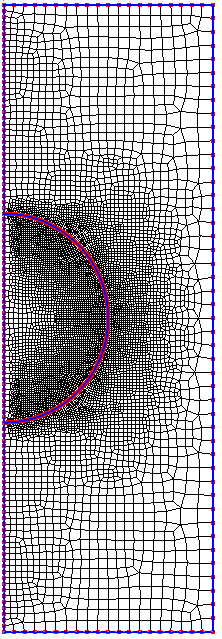
\includegraphics[scale=0.55]{mesh/meshfar}
	\end{minipage}%
	\begin{minipage}{.60\paperwidth}
		%\centering
		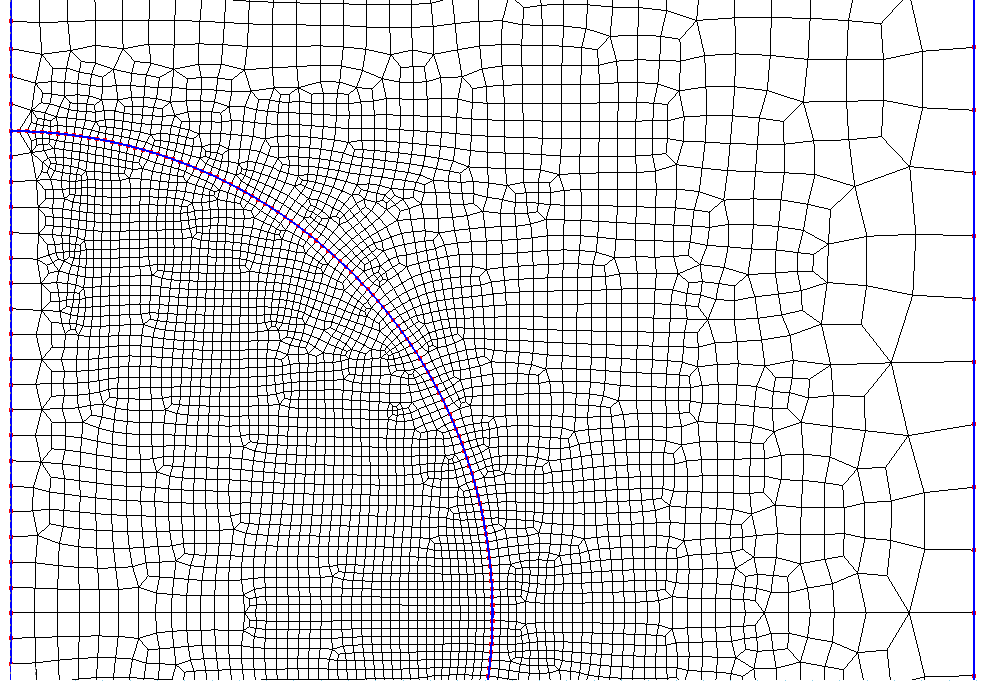
\includegraphics[scale=0.50]{mesh/mesh3}
	\end{minipage}
}
\caption{Ejemplo de malla. Dominio completo (izquierda) y detalle (derecha). La célula tiene forma de semicírculo dado que se usan coordenadas cilíndricas. Los elementos de la membrana son los más pequeños y no se alcanzan a ver.}
\end{figure}


\begin{figure}
	
\includegraphics[width=\textwidth]{mesh/membrana}
	\caption{Detalle de la malla cerca de la membrana. Los líneas dobles corresponden a elementos de la membrana celular, los elementos de la izquierda corresponden al interior de la célula y los de la derecha al exterior.}
	\label{fig:mesh-membrana}
\end{figure}


Las mallas utilizadas tienen entre 7500 y 8900 elementos y representan un dominio de hasta 150 \si{\micro\metre} de alto y hasta 50 \si{\micro\metre} de ancho con una célula cuyo radio varía entre 10 y 50 \si{\micro\metre} y con una membrana de 5 \si{\nano\metre} de espesor. Para modelar la membrana se crearon tres arcos separados a 2.5 \si{\nano\metre} de distancia, que fueron divididos en 192 partes en la dirección del ángulo polar. De esta manera se obtiene una membrana con dos elementos en la dirección radial. Los electrodos se modelaron dentro del dominio, en los bordes superior e inferior.

También se usó \nombre{Python} como lenguaje secundario, para ayudar en la generación de mallas, la interpretación de los datos de salida obtenidos en las simulaciones y la generación de gráficos, haciendo uso de la librería \nombre{matplotlib} \cite{matplotlib}. El programa lee los parámetros de ejecución de un archivo \texttt{input.in} y graba periódicamente resultados de potencial y campo eléctrico, potencial transmembrana, densidad y radios de poros en la membrana celular, concentraciones de las especies y valores de pH en diferentes archivos de salida.

%\clearpage

\subsection*{Escalabilidad}

El código implementado contiene partes que corren en paralelo implementadas con \nombre{OpenMP} para mejorar así los tiempos de ejecución.\\

\textbf{OpenMP} es una API (interfaz de programación de aplicaciones) que permite implementar con facilidad código paralelo con múltiples hilos de ejecución y memoria compartida \cite{quinn}. Consta de un conjunto de directivas para el compilador llamadas \textit{pragmas} y se puede utilizar en programas de Fortran, \texttt{C} y \texttt{C++}. Una de las principales ventajas de \nombre{OpenMP} contra otros paradigmas de paralelización como el pasaje de mensajes, es que con OpenMP es muy fácil convertir código serial a paralelo. Por ejemplo para convertir un ciclo serial que consume mucho tiempo de ejecución a uno paralelo suele bastar con agregar unos pocos \textit{pragmas} al código. Con el modelo de pasaje de mensajes, en cambio, sería necesario reescribir gran parte de la lógica del programa, ya que los diferentes procesos no compartirían memoria y necesitarían enviarse mensajes explícitamente. Como desventaja se tiene que es necesario que todos los núcleos involucrados en el cómputo compartan la misma memoria, lo cual impide utilizar clústers de computadoras limitando la paralelización que es posible obtener. Esto no es un problema en este trabajo, ya que se utilizan mallas bidimensionales relativamente pequeñas y que gran parte del código es serial, y por lo tanto no se obtendría una mejora significativa con una cantidad muy grande de procesos ejecutando en paralelo.\\

%TODO se podría explicar que pragmas se usan en el código

Para medir la mejora obtenida al utilizar varios hilos de ejecución se utilizan las medidas de \textit{speedup} y \textit{eficiencia}. Se define speedup como $S = T_s / T_p$ donde $T_s$ es el tiempo de ejecución serial (con un solo proceso o hilo) y $T_p$ el tiempo de ejecución paralelo \cite{pacheco}. La eficiencia en cambio es $E = S / p$ donde $S$ es el speedup y $p$ la cantidad de procesos o hilos \cite{pacheco}.\\

En la tabla \ref{tab:escala} se encuentran medidas de los tiempos de ejecución, speedup y eficiencia de una simulación similar a las realizadas en el capítulo \ref{chap:acoplado}, usando entre 1 y 4 hilos de ejecución. Se puede ver que los mejores tiempos se obtuvieron con 4 threads, pero sin embargo el speedup es apenas mayor al obtenido con 2 threads, y la eficiencia es mucho menor. Se puede concluir que el programa escala correctamente para 2 threads, pero no mejora notablemente al agregar más hilos de ejecución, e incluso empeora los tiempos de ejecución al pasar de 2 a 3 hilos. La baja escalabilidad puede deberse a que solo una fracción del código corre en paralelo (el armado de matrices del cálculo del potencial eléctrico y el cálculo de las concentraciones de especies), mientras que la mayor parte es serial (los cálculos relacionados a los poros y la factorización de matrices para el potencial eléctrico).

\begin{table}
    \centering
	\begin{tabular}{ c | c c c c }              
		& 1 thread & 2 threads & 3 threads & 4 threads \\
		\hline
		Tiempo [\si{\second}] & 1995 & 1331 & 1489 & 1233 \\
		Speedup & 1 & 1.50 & 1.34 & 1.63 \\
		Eficiencia & 100\% & 74.9\% & 44.7\% & 40.5\% \\
	\end{tabular}
    \caption{Tiempos de ejecución para un pulso de 5 \si{\milli\second} y una malla de 8899 nodos corriendo en un CPU intel i3 2100 a 3.10 GHz con capacidad para 4 threads}
    \label{tab:escala}
\end{table}
